\section{内容}
本実験では\figref{fig:ネットワーク図}のネットワークを作成する.
ルーティングの設定やNAPTは\figref{fig:ネットワーク図}の\texttt{Ruter5}に行う.
\begin{figure}
    \centering
    \begin{framed}
    \begin{tikzpicture}
        \newcommand{\rt}{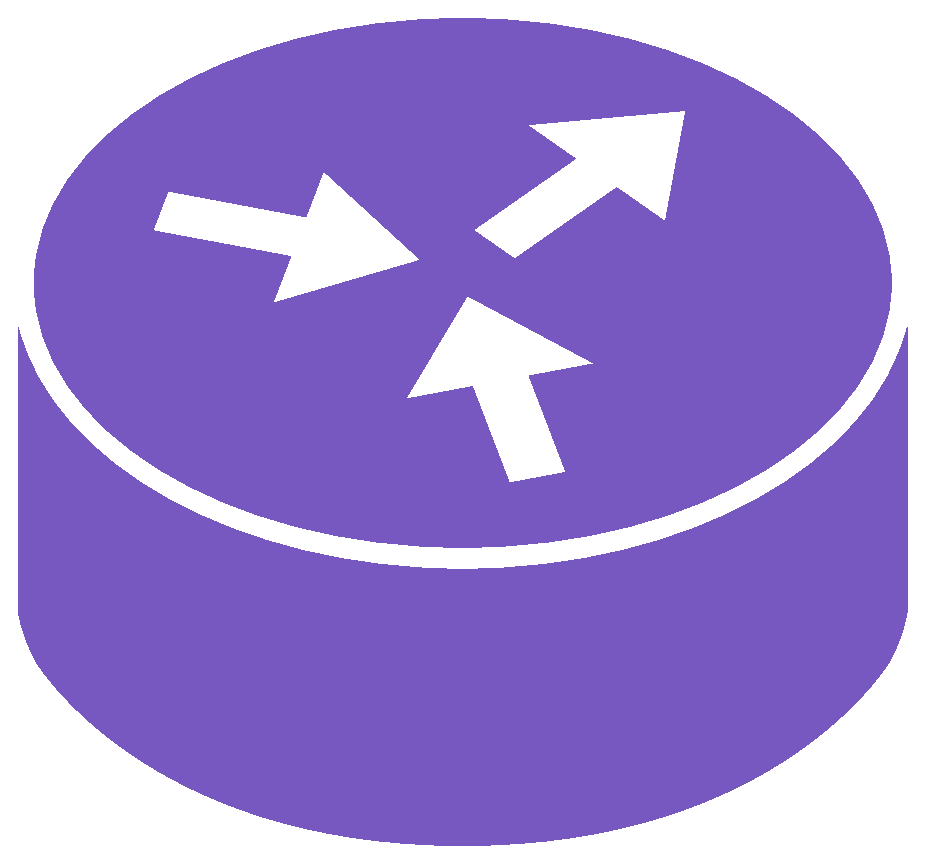
\includegraphics[keepaspectratio,width=2cm]{../network_iconset/router_01_nb.pdf}}
        \newcommand{\host}{
\includegraphics[keepaspectratio,width=1cm]{../network_iconset/laptop_nb.pdf}}
        \node(rtA){\rt};
        \node[right=3cm of rtA.east](rtB){\rt};
        \coordinate (O) at ($(rtB.east)+(2.5cm,0)$);
        \node[above=2cm of O](hostA){\host};
        \node[above=1cm of O](hostB){\host};
        \node[below=1cm of O](hostC){\host};
        \node[below=2cm of O](hostD){\host};
        \coordinate (O1) at ($(rtB.east)+(1cm,.2cm)$);
        \coordinate (O2) at ($(rtB.east)+(1cm,-.2cm)$);
        \draw[ultra thick]{
            ($(rtA)!0.5!(rtB)$)--($(rtA)!0.5!(rtB)+(0,3cm)$)--($(rtA)!0.5!(rtB)+(1cm,3cm)$)
            ($(rtA)!0.5!(rtB)+(0,1cm)$)--($(rtA)!0.5!(rtB)+(1cm,1cm)$)
            ($(rtA)!0.5!(rtB)+(0,2cm)$)--($(rtA)!0.5!(rtB)+(1cm,2cm)$)
            ($(rtA.west)+(-.5cm,0)$)node[left,ellipse,fill=gray!30]{\scriptsize インターネット}--(rtA)
            (rtA)--(rtB)node[midway,ellipse,fill=black,text=white](bb){\scriptsize バックボーン}
            (rtB.east|-O1)--(O1)--($(O1|-hostA.west)+(0,.5cm)$)
            (rtB.east|-O2)--(O2)--($(O2|-hostD.west)+(0,-.5cm)$)
            (hostA)--(O1|-hostA.west)
            (hostB)--(O1|-hostB.west)
            (hostC)--(O2|-hostC.west)
            (hostD)--(O2|-hostD.west)
        };
        \draw[ultra thick,dashed]{
            ($(rtA)!0.5!(rtB)+(1cm,1cm)$)--($(rtA)!0.5!(rtB)+(1.5cm,1cm)$)
            ($(rtA)!0.5!(rtB)+(1cm,2cm)$)--($(rtA)!0.5!(rtB)+(1.5cm,2cm)$)
            ($(rtA)!0.5!(rtB)+(1cm,3cm)$)--($(rtA)!0.5!(rtB)+(1.5cm,3cm)$)
        };
        \foreach \u \v in{A/server,B/client,C/server,D/client}{
                \node[right=-.1cm]at(host\u.east)(cp\u){\footnotesize\texttt{\v}};
            }
        \node[below=.3cm,text=white]at(rtB){\texttt{router5}};
        \node[below=.3cm,text=white]at(rtA){\scriptsize メインルータ};
        \node[fit={(hostA)(hostB)(cpA)(cpB)},draw,dotted,thick,rounded corners](sg1){};
        \node[fit={(hostC)(hostD)(cpC)(cpD)},draw,dotted,thick,rounded corners](sg2){};
        \begin{scope}[on background layer]
            \node[below]at(sg1.south){5C班LAN};
            \node[above]at(sg2.north){5i班LAN};
            \node[below]at(bb.south){\scriptsize\texttt{192.168.0.0/24}};
            \node[left]at($(O1|-hostA.west)!0.5!(O1|-hostB.west)$){\scriptsize\texttt{172.21.26.0/24}};
            \node[left]at($(O2|-hostC.west)!0.5!(O2|-hostD.west)$){\scriptsize\texttt{172.21.15.0/24}};
            \node[left,text=gray]at(O1|-hostA.west)(cpA){\scriptsize\texttt{172.21.26.2}};
            \node[left,text=gray]at(O1|-hostB.west)(cpB){\scriptsize\texttt{172.21.26.3}};
            \node[left,text=gray]at(O2|-hostC.west)(cpC){\scriptsize\texttt{172.21.15.2}};
            \node[left,text=gray]at(O2|-hostD.west)(cpD){\scriptsize\texttt{172.21.15.3}};
            \node[right,text=gray]at(O1)(capO1){\scriptsize\texttt{172.21.26.1}};
            \node[right,text=gray]at(O2)(capO2){\scriptsize\texttt{172.21.15.1}};
            \node[below=1cm of rtB.west,text=gray](ipbb){\scriptsize\texttt{192.168.0.59}};
            \draw[black,fill=black](rtB.west)circle[radius=.5mm]node(A){};
            \draw[-latex,gray](ipbb)--(A);
            \node[below=1cm of rtA.east,text=gray](ipbb){\scriptsize\texttt{192.168.0.9}};
            \draw[black,fill=black](rtA.east)circle[radius=.5mm]node(A){};
            \draw[-latex,gray](ipbb)--(A);
            \draw[black,fill=black](rtB.east|-O1)circle[radius=.5mm]node(A){};
            \draw[-latex,gray](capO1)to[bend right=30](A);
            \draw[black,fill=black](rtB.east|-O2)circle[radius=.5mm]node(A){};
            \draw[-latex,gray](capO2)to[bend left=30](A);
            \foreach \u in{A,B,C,D}{
            \draw[black,fill=black](host\u.west)circle[radius=.5mm]node(\u){};
            }
            \foreach \u in{A,C}{
                    \draw[-latex,gray](cp\u)to[bend left=30](\u);
                }
            \foreach \u in{B,D}{
                    \draw[-latex,gray](cp\u)to[bend right=30](\u);
                }
        \end{scope}
        \coordinate (A) at ($(rtA)!0.5!(rtB)+(0cm,2.5cm)$);
        \coordinate (B) at (rtA |- A);
        \node at (B)(rtTA){\rt};
        \node[below=.3cm,text=white]at(rtTA){\scriptsize TA用ルータ};
        \node[left=1cm of rtTA.west](hostTA){\host};
        \node[below] at (hostTA.south){\scriptsize TA用\texttt{server}};
        \draw[ultra thick]{
            (A)--(rtTA)
            (rtTA)--(hostTA)
        };
        \draw[black,fill=black](rtTA.east)circle[radius=.5mm]node(rtTA){};
        \draw[black,fill=black](hostTA.east)circle[radius=.5mm]node(hostTA){};
        \node[below=1cm of rtTA,text=gray](caprtTA){\scriptsize\texttt{192.168.0.239}};
        \draw[-latex,gray](caprtTA)--(rtTA);
        \node[above=.5cm of hostTA](caprtAH){\scriptsize\texttt{172.21.33.0/24}};
    \end{tikzpicture}
\end{framed}

    \caption{論理ネットワーク図(L2スイッチは省略)}
    \label{fig:ネットワーク図}
\end{figure}
\subsection{スイッチの設定}
コンソールへ接続し,L2スイッチにIPアドレスを付与する.(\texttt{telnet}での操作を可能にするため.)
スパニングツリー機能を停止した後VLANを用いて,1台のスイッチ内に3つのセグメント(\textbf{デフォルトセグメント},\textbf{5C班セグメント},\textbf{5i班セグメント})を作成する.
\subsection{ルータの初期設定}
コンソールへ接続し,バックボーンのIPアドレス,5C班のネットワークアドレス,5i班のネットワークアドレスと各サブネットマスクを決定する.
ルータへIPアドレスを付与した後,ルーティングテーブルを作成する.
動的ルーティングはOSPFを用い,デフォルトルートとしてメインルータ(\texttt{192.168.0.9})を,TA班用への経路を静的経路として設定する.
\subsection{ホストのネットワーク設定}
サーバのIPアドレス,DNSゾーンの設定,ApacheのIPアドレス制限の設定を更新する.それに伴い,クライアントのネットワーク設定も更新する.
\subsection{NAPT・ポートフォワーディングの設定}
5C班LAN(内部)からバックボーン(外部),そして外部から内部へのアクセスを,以下のように\texttt{Ruter5}へ設定する.
\begin{itemize}
    \item 内部から外部へは,動的NAPTを用いて任意のアクセスを許可する.
    \item 外部からサーバ以外ホストへのアクセスを禁止する.
    \item 外部からサーバへ,静的NAPTを用いて以下のアクセスを許可する.
          \begin{multicols}{2}
              \begin{itemize}
                  \item DNS(TCP,UDP)\\宛先ポート53番,転送先ポート53番
                  \item Web(TCP)\\宛先ポート80番,転送先ポート80番
                  \item SMTP(TCP)\\宛先ポート25番,転送先ポート25番
                  \item SSH(TCP)\\宛先ポート8022番,転送先ポート22番
              \end{itemize}
          \end{multicols}
\end{itemize}
